\begin{figure}[!htbp]
\centering
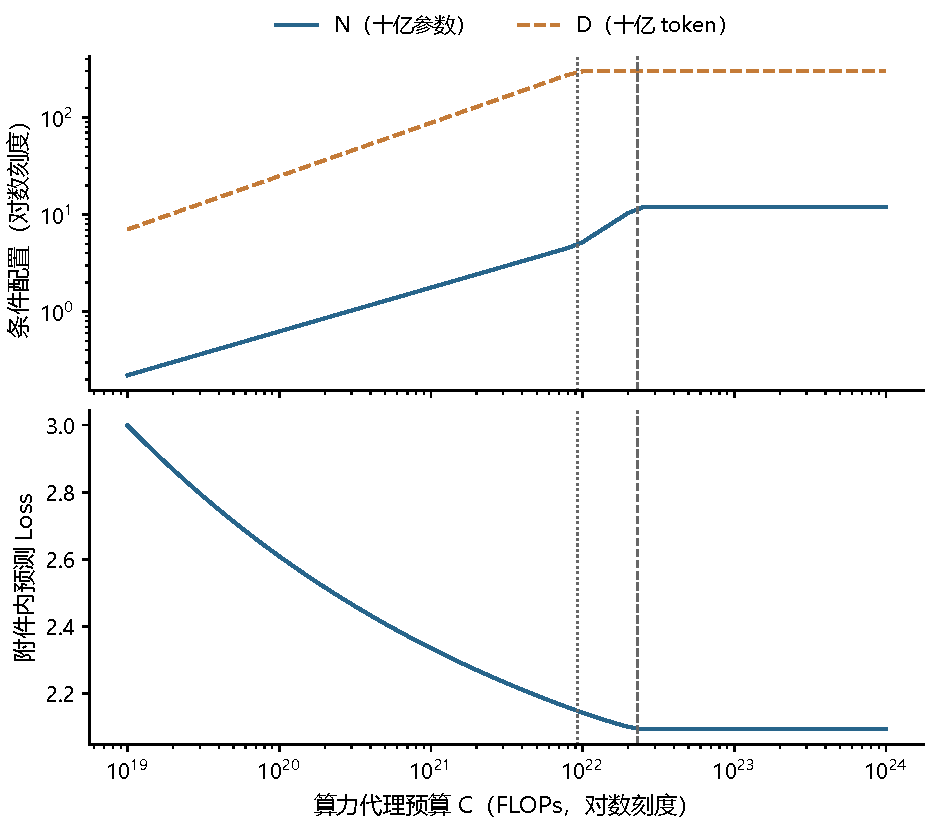
\includegraphics[width=15cm]{06_results/figures/round6/FIG-Q3-R6-001.pdf}
\caption{基线预算路径：虚线为统计支持边界触发，后段平台不代表现实扩展失效。}
\end{figure}
\begin{figure}[!htbp]
\centering
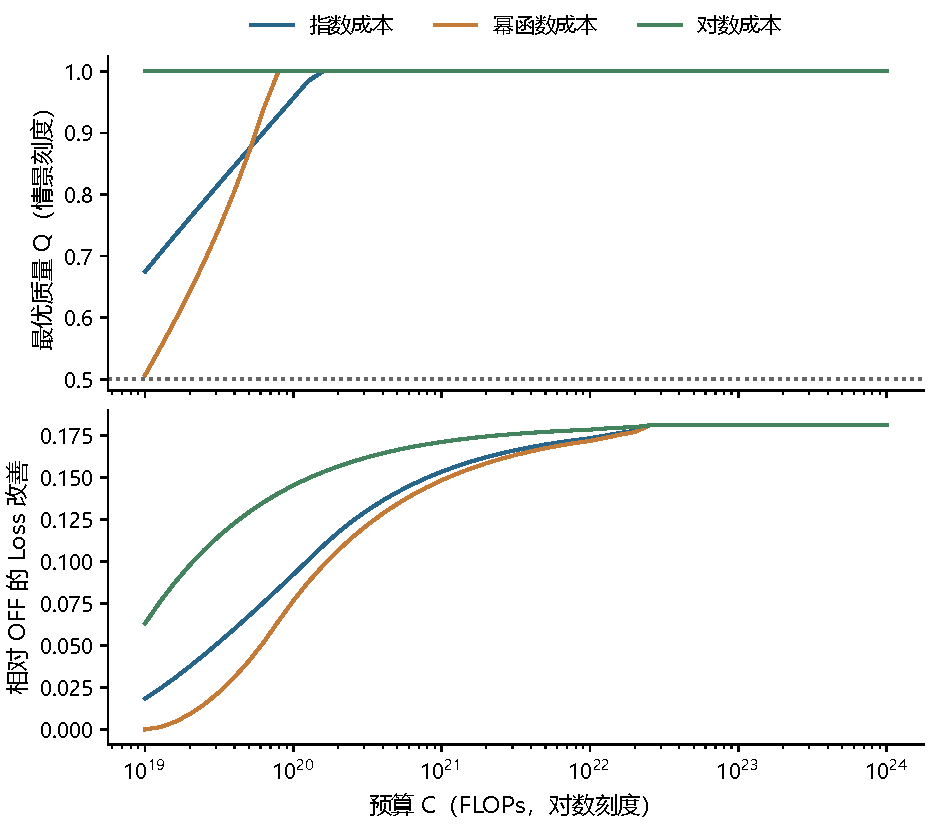
\includegraphics[width=15cm]{06_results/figures/round6/FIG-Q3-R6-002.pdf}
\caption{同一REFERENCE质量收益假设下，三类题面成本导致不同质量投入路径。}
\end{figure}
\begin{figure}[!htbp]
\centering
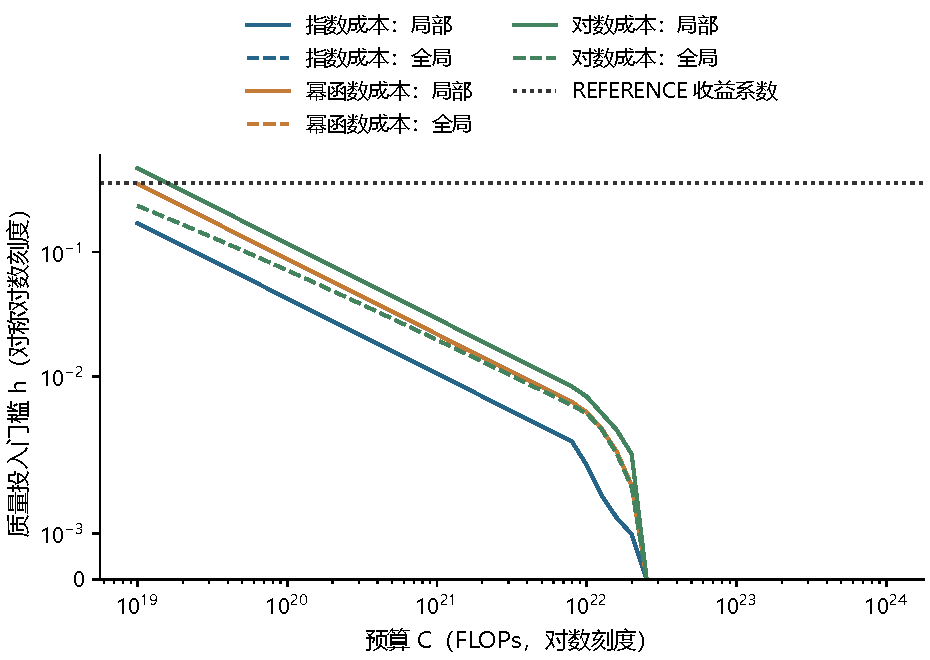
\includegraphics[width=15cm]{06_results/figures/round6/FIG-Q3-R6-003.pdf}
\caption{对数成本的局部与全局质量激活门槛分离，不能只用一阶条件判断投入。}
\end{figure}
\begin{figure}[!htbp]
\centering
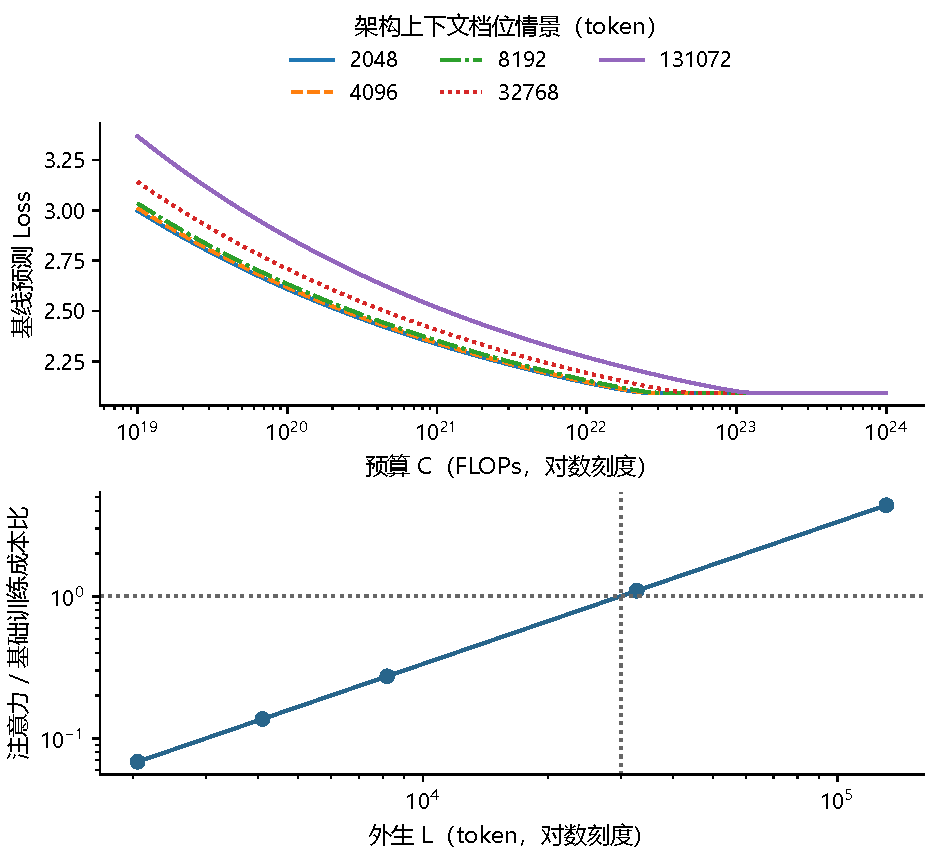
\includegraphics[width=15cm]{06_results/figures/round6/FIG-Q3-R6-004.pdf}
\caption{C7最大上下文档位仅用作外生情景；30000是成本代理等值点。}
\end{figure}
\begin{figure}[!htbp]
\centering
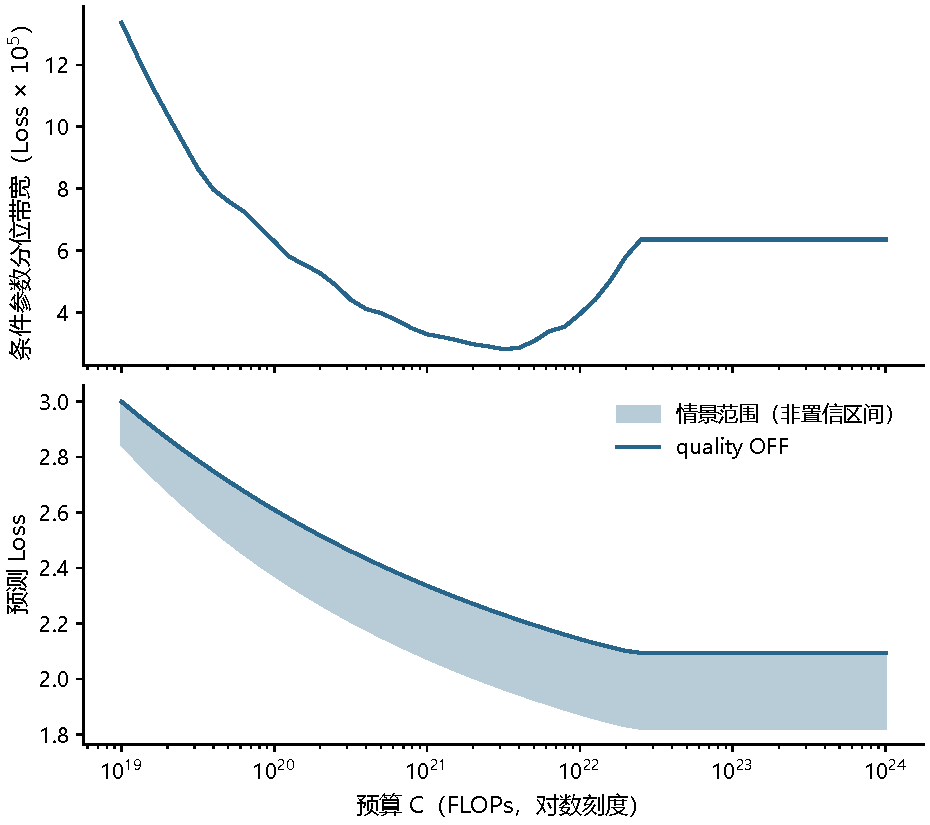
\includegraphics[width=15cm]{06_results/figures/round6/FIG-Q3-R6-005.pdf}
\caption{给定附件的参数带极窄，机制情景范围更宽；两者均不保证外部覆盖。}
\end{figure}
\begin{figure}[!htbp]
\centering
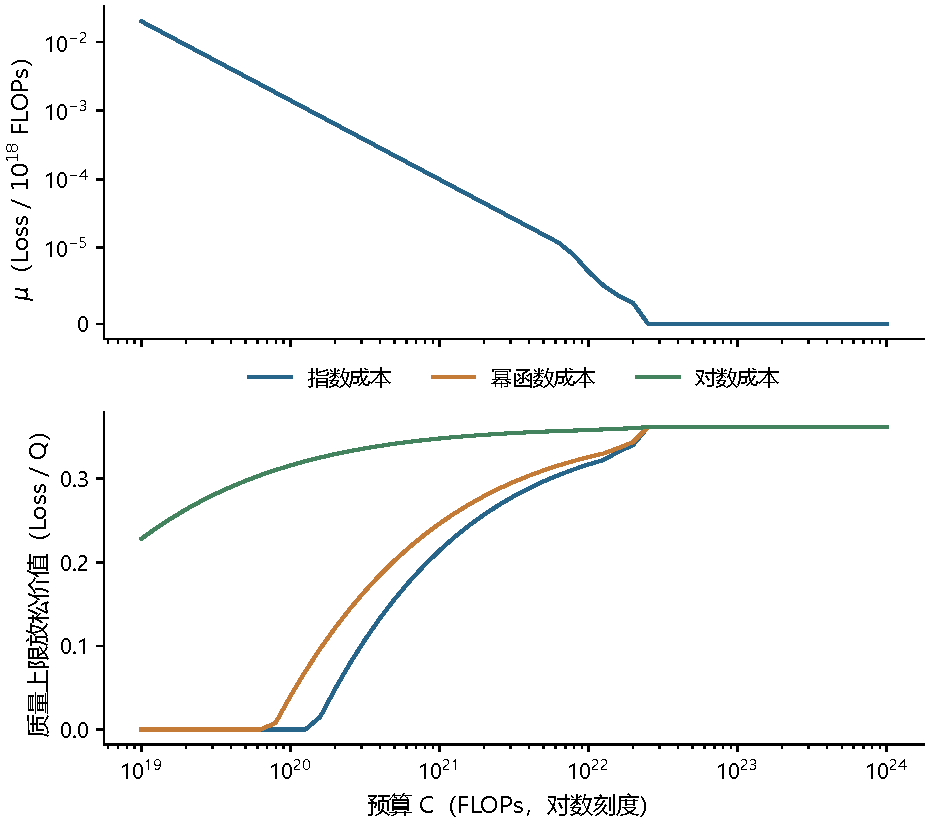
\includegraphics[width=15cm]{06_results/figures/round6/FIG-Q3-R6-006.pdf}
\caption{预算影子价在统计支持饱和后为零；质量上限价值仍只属收益假设。}
\end{figure}
